\documentclass[a4paper, 11pt]{article}
\usepackage[left=2cm,text={17cm, 24cm},top=3cm]{geometry}
\usepackage[czech]{babel}
\usepackage[IL2]{fontenc}
\usepackage[utf8]{inputenc}
\usepackage{times}
\usepackage{graphicx}
\usepackage{pdflscape}
\usepackage{picture}

\usepackage{url}
\DeclareUrlCommand\url{\def\UrlLeft{<}\def\UrlRight{>} \urlstyle{tt}}

\begin{document}
\newcommand{\myuv}[1]{\quotedblbase #1\textquotedblleft}

\thispagestyle{empty}
\onecolumn
\begin{center}
\Huge
\textsc{Vysoké učení technické v~Brně\\\huge{Fakulta Informačních Technologií}}

\LARGE
\vspace{\stretch{0.382}}
Modelování a Simulace\,--\,Projekt, téma č.2

\Huge{Distribuční centrum}
\vspace{\stretch{0.618}}
\end{center}
{\LARGE 29.11.2018 \hfill
Matěj Hrabal, Patrik Holop}
\newpage
\setcounter{page}{1}
\section{Úvod}
V rámci projektu jsme se rozhodli vytvořit simulační model\cite[slide 9]{IMS} distribučního centra firmy [REDACTED], které se nachází na adrese [REDACTED]. Cílem bylo experimentováním se simulačním modelem zjistit, zda je možné práci distribučního centra vylepšit pomocí drobných úprav areálu a také zjistit dopady změn plánovaných samotnou firmou. Pro projekt bylo nutné nastudovat problematiku zpracování logistických požadavků, dopravních vozidel a pracovní procesy v jednotlivých částech areálu distribučního centra.
\subsection{Autoři a odborní konzultanti}
Autoři práce jsou Matěj Hrabal (xhraba12) a Patrik Holop (xholop01).
Práce byla konzultována přímo v distribučním centru firmy [REDACTED] s několika zaměstnanci a s panem Miroslavem Martincem, který se několik let živil jako řidič nákladního vozidla.
\subsection{Ověřování validity modelu}
Před tvorbou modelu byly analyzovány statistiky firmy [REDACTED] výsledky získané konzultacemi a z jejich oficiální webové stránky. Hodnoty, které se v statistikách nenacházeli (např. časové údaje) byly měřeny autory projektu přímo v areálu distribučního centra po dobu několika hodin. Výsledky experimentů odpovídali statistikám poskytnutým zaměstnanci firmy a model jsme určili jako validní\cite[slide 37]{IMS}.

\section{Rozbor tématu a použitých metod/technologií}
Provoz distribučního centra firmy [REDACTED] funguje tak, že firemní vozy přiváží do centrálního skladu různé druhy výrobků na EUR paletách\cite{PAL} pro uskladnění, které zůstávají uloženy na skladě do té doby, než je jeden z firemních vozů odveze na požadované místo (např. obchodní řetězec).
Požadavky na jednotlivé dovozy i odvozy mají předem přidelený typ vozu, který je musí provést. Odstavená vozidla se nacházejí v přední části areálu. Aby se jednotlivá vozidla dostala ke skladu, musí obejít danou budovu a projet objezdovou cestou kolem centrální budovy. Logistické centrum má oddělené vykladácí a nakládací plošiny. Když od areálu přijede naložený vůz, nejdřív zaparkuje na odděleném parkovišti v přední části a do skladu se snaží dostat až po zajištění vykládacího místa.\\

\noindent Normální rozdělení pravděpodobnosti jsou uvedena ve tvaru $\mathcal{N}(\mu,\,\sigma^{2})\,$, exponenciální rozložení pravděpodobnosti ve tvaru $\exp$(střední hodnota).\\


\noindent Hodnoty získané měřením a konzultacemi:
\begin{itemize}
\item Doba parkování k plošinám: $\mathcal{N}(3 min, 400s)$
\item Doba výjezdu ze skladu: $\mathcal{N}(60s, 100s)$
\item Doba parkování v lokálním parkovišti: $\mathcal{N}(60s, 100s)$
\item Doba nakládání a vykládání vozů: $\mathcal{N}(15s, 1s)$
\item Doba průjezdu úzkým objezdem kolem budovy: $\mathcal{N}(12s, 1s)$
\item Doba průjezdu odjezdovou cestou z areálu: $\mathcal{N}(15s, 1s)$
\item Doba odstavení vozů: $\mathcal{N}(60s, 100s)$
\item Doba uzavření	nákladního prostoru: $15s$
\end{itemize}

\newpage
\noindent Hodnoty získané z webové stránky\cite{LAL}:
\begin{itemize}
\item Kapacita skladu: 5000 EUR palet
\item Celkový počet vozů: 50
\end{itemize}

\noindent Hodnoty získané ze statistik firmy:
\begin{itemize}
\item Typy vozů a přibližné pravděpodobnosti požadavku na jízdu daného typu: \\
Iveco (20\%), Volvo (25\%), Ford (25\%), Man (20\%), Man - druhý typ (10\%)\\
Pravděpodobnost je pro dovozní i odvozní jízdy stejná.

\item Statistiky naložení jednotlivých vozů

\item Doba mezi jednotlivými požadavky na přesun:\\
Dovozní jízda (den): $\exp(1200s)$\\
Dovozní jízda (noc): $\exp(2400s)$\\
Odvozní jízda (den): $\exp(1400s)$\\
Odvozní jízda (noc): $\exp(1800s)$\\
Denní hodnoty jsou podpořeny také osobním měřením.

\item Doba jízdy strávená vozem mimo areálu: $\mathcal{N}(3h, 0.04h)$
\item Počet nakládacích plošin: 4
\item Počet vykládacích plošin: 2
\end{itemize}

\subsection{Popis použitých postupů}
Projekt byl napsán v jazyce C++ s využitím knihovny SIMLIB\cite{SIML}. Jazyk C++ byl vybrán, protože společně s jazykem C se jednalo o jediné povolené programovací jazyky pro psaní projektu\cite{Zadani} a také umožnuje objektově orientovaný návrh programu. Petriho síť byla navržená v programu GreatSPN Editor, který nabízí všechny potřebné funkce pro vytvoření přehledné Petriho sítě.

\subsection{Popis původu použitých metod/technologií}
K projektu byla využita knihovna SIMLIB stažená z oficiálních stránek knihovny SIMLIB\cite{SIML}. Pro překlad byl zvolen překladač g++\cite{G}. Dále byly použity standardní knihovny jazyka C++. Pro vytvoření Petriho sítě byl použit program GreatSPN Editor stažený z oficiálních stránek tohoto editoru\cite{SPN}.

\section{Koncepce}
\subsection{Modelářská témata}
Práce distribučního centra vypadá následovně:
Distribuční centrum má celkem 5 různých typů vozidel pro náklad. Průměrné hodnoty naložení jednotlivých typů se liší. Kapacitu skladu počítáme v EUR paletách\cite{PAL}. Do distribučního centra přichází různé požadavky na odvoz a dovoz palet. Tyto požadavky jsou vyřizovány dostupným vozidlem vhodným pro daný požadavek.\\
\indent Pokud vozidlo dostává požadavek k přivezení počtu palet k uskladnění v distribučním centru, tak nejprve vyrazí pro náklad z parkoviště, po naložení nákladu se vrátí zpět do distribučního centra, kde zaparkuje na vyhrazeném parkovišti, kde obsadí jednu z vykládacích plošin (nebo počká na uvolnění plošiny na parkovišti, není-li žádná vykládací plošina volná). Může se stát, že vyhrazené parkovište je plné. V takém případe odjede na vzdálené parkovište mimo areál distribučního centra. Tento případ sice v praxi ješte nenastal, ale je nutné ho modulovat kvůli podstatě konkrétních experimentů. Na vykládací plošině vyloží svůj náklad a řidič svůj vůz odstaví na původním místě.\\\indent V případě požadavku na odvoz palet je vozidlo nejprve posláno k jedné z nakládacích plošin (popřípadě čeká na její uvolnění na parkovišti), u rampy jsou na vozidlo naloženy palety, a tyto palety jsou odvezeny na místo určení. Poté se vozidlo vrací zpět a je připraveno přijmout další požadavek.

Zjednodušená Petriho síť pro odvoz modeluje jednotlivé generování požadavků na odvoz určitého počtu EUR palet na místo určení. Oproti simulačnímu modelu byly provedeny změny u některých časových položek, kdy přímo na sebe navazující časové úkony (Např. zavírání dveří vozidla a odjezd od rampy) byly zakresleny jako jedno čekání. Dále byl v síti zjednodušen výběr vozidla, protože každý typ má jinou průměrnou obsazenost EUR paletami. V Petriho síti je tento údaj vyznačen proměnnou \myuv{N}. Vykládaní a nakládaní palet do skladu je také zjednodušeno společně s obsazováním odjezdové cesty, která je vyznačena pouze časovým údajem.\\

\noindent V Petriho síti jsou časové jednotky uvedené v sekundách, pokud není uvedeno jinak.

\begin{figure}[ht!]
\begin{center}
\includegraphics[scale=0.2]{petri1.eps}
\caption{Zjednodušena Petriho síť pro odvoz palet z distribučního centra}
\end{center}
\end{figure}
\newpage
\begin{figure}[ht!]
\begin{center}
\includegraphics[scale=0.2]{petri2.eps}
\caption{Zjednodušena Petriho síť pro dovoz palet z distribučního centra}
\end{center}
\end{figure}
U zjednodušené Petriho sítě pro dovoz je změna chování v tom, že se do skladu dováží EUR palety výrobků (pokud je ve skladu místo).

\section{Architektura simulačního modelu/simulátoru}
Celá simulace je inicializována v čase 00:00. Na konkrétním dni nezáleží (viz. sekce Modelářská témata). Třída \emph{SpusteniSimulace} v tomto čase inicializuje úvodní naplnění parkoviště a skladu. Dále se do kalendáře přidá čas zapnutí procesu, který přepíná mezi denní a noční směnou tak, aby denní směna začala v 8 hodin a poté se střídala po 12 hodinách (Třída \emph{Směny}). Směna rozhoduje, jak často se generují procesy odvozu a dovozu nákladu. Spouštění těchto procesů má na starost Třída \emph{GeneratorJizd}. Tyto třídy spouštějí proces \emph{JizdaVozu}, který obsahuje jednotlivé úkony, které je potřeba vykonat při dovozu a odvozu nákladu.

\section{Podstata simulačních experimentů a jejich průběh}
\subsection{Postup experimentování}
V rámci experimentování jsme se snažili držet reality a pomocí pouze drobných úprav areálu vylepšit celkový provoz distribučního centra. Za drobnou úpravu považujeme např. přestavbu jednoho parkovacího místa na nakládací plošinu, zmenšení skladiště se současným přidáním parkovacích míst, popřípadě přikoupení plochy pro další parkovací místa.

\subsection{Dokumentace jednotlivých experimentů}
\subsubsection{Experiment 1}
Experiment číslo 1 byl proveden se základními neoptimalizovanými hodnotami, které lze nalézt v kapitole \myuv{Rozbor tématu a použitých metod-technologií}. Byly sledovány stavy jednotlivých front a skladů. Všechny výsledky byli podle očekávaní. Jelikož bylo průměrné vytížení jednotlivých vozů nízké, nastaly výjimečné situace, kdy délky front pro jednotlivé typy dosahovali až hodnoty 5.
Také výjimečně vznikla fronta pro vykládací plošinu. Obě tyto hodnoty můžou ovlivňovat výjimečný dlouhý čas vyřizovaní objednávek (nad 16000s). Firma ale neví, zda se vyplatí investovat do přidání vykládacích plošin nebo přidání vozů.\\

\begin{center}
\noindent Maximální délka fronty pro plošiny:\\
\indent Vykládací plošina: 4\\
\indent Nakládací plošina: 1\\
Maximální obsazení parkovište: 4\\
\end{center}

\begin{center}
\begin{tabular}[h!]{|c|c|}
\hline
Typ vozu & Maximální délka fronty pro daný typ \\ \hline
0 & 5 \\ \hline
1 & 5 \\ \hline
2 & 5 \\ \hline
3 & 2 \\ \hline
4 & 0 \\ \hline
\end{tabular}
\end{center}

\begin{figure}[h!]
\begin{center}
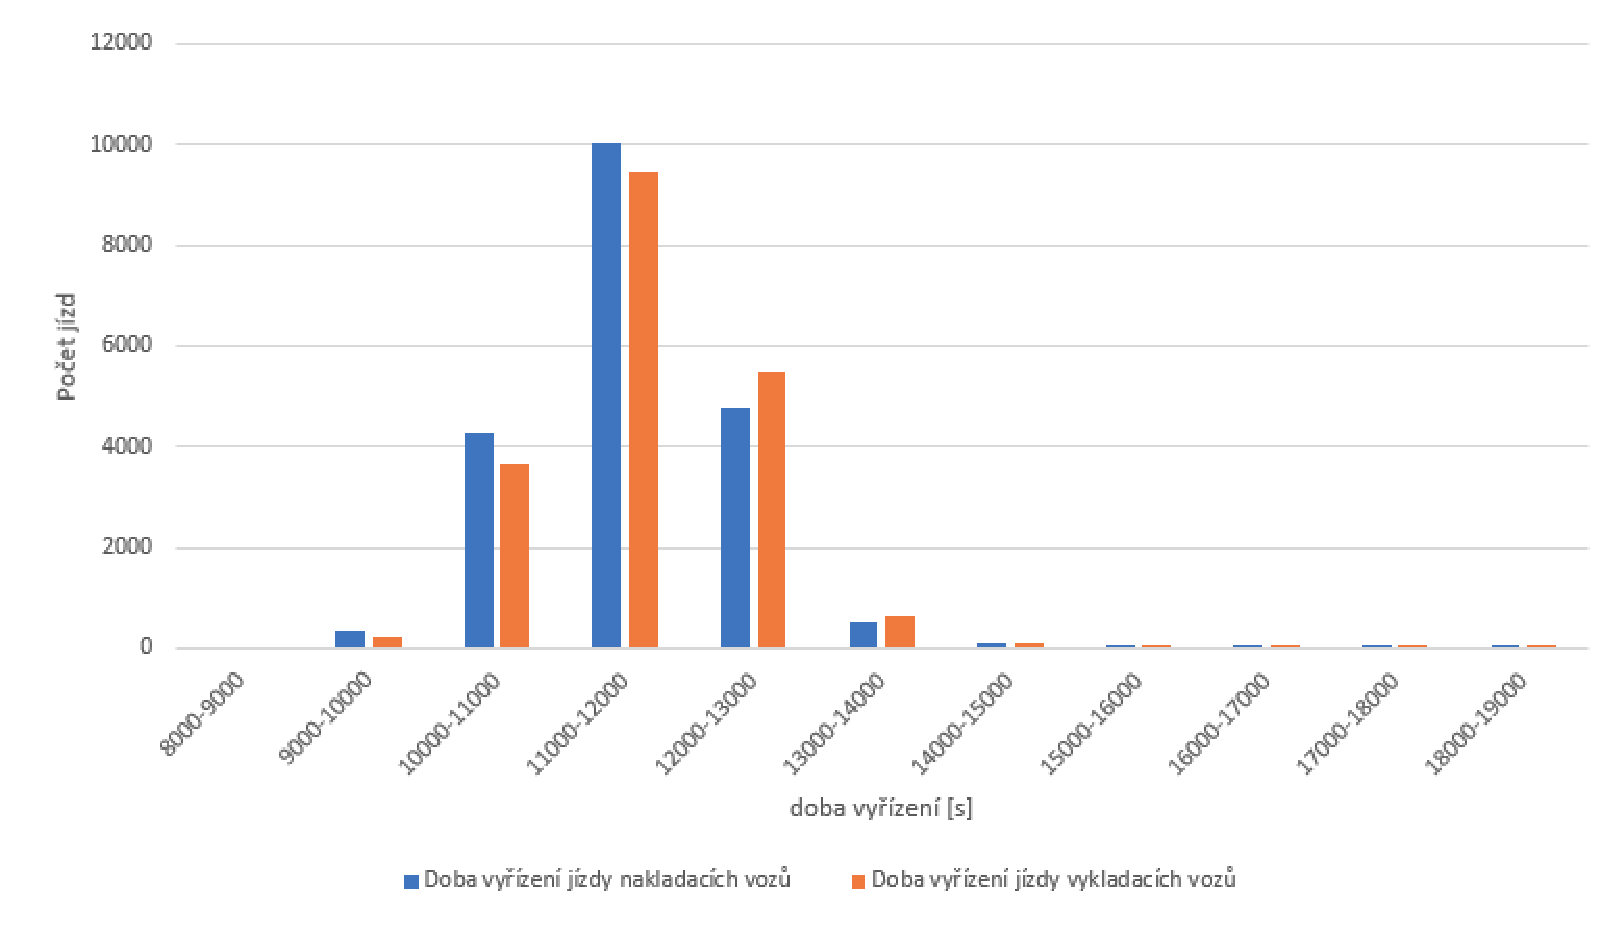
\includegraphics[scale=0.5]{exp1.eps}
\caption{Graf vyřizování jízd experimentu 1}
\end{center}
\end{figure}
\vspace{20pt}

\newpage
\subsubsection{Experiment 2}
\noindent V experimentu číslo 2 jsme experimentovali se zvyšováním počtu vykládacích plošin za účelem snížení výjimečne dlouhých vyřizování. Jak lze vidět na obrázku 4, přídaní vykládacích plošin nemělo na odstranění těchto situací vliv.

\begin{figure}[h!]
\begin{center}
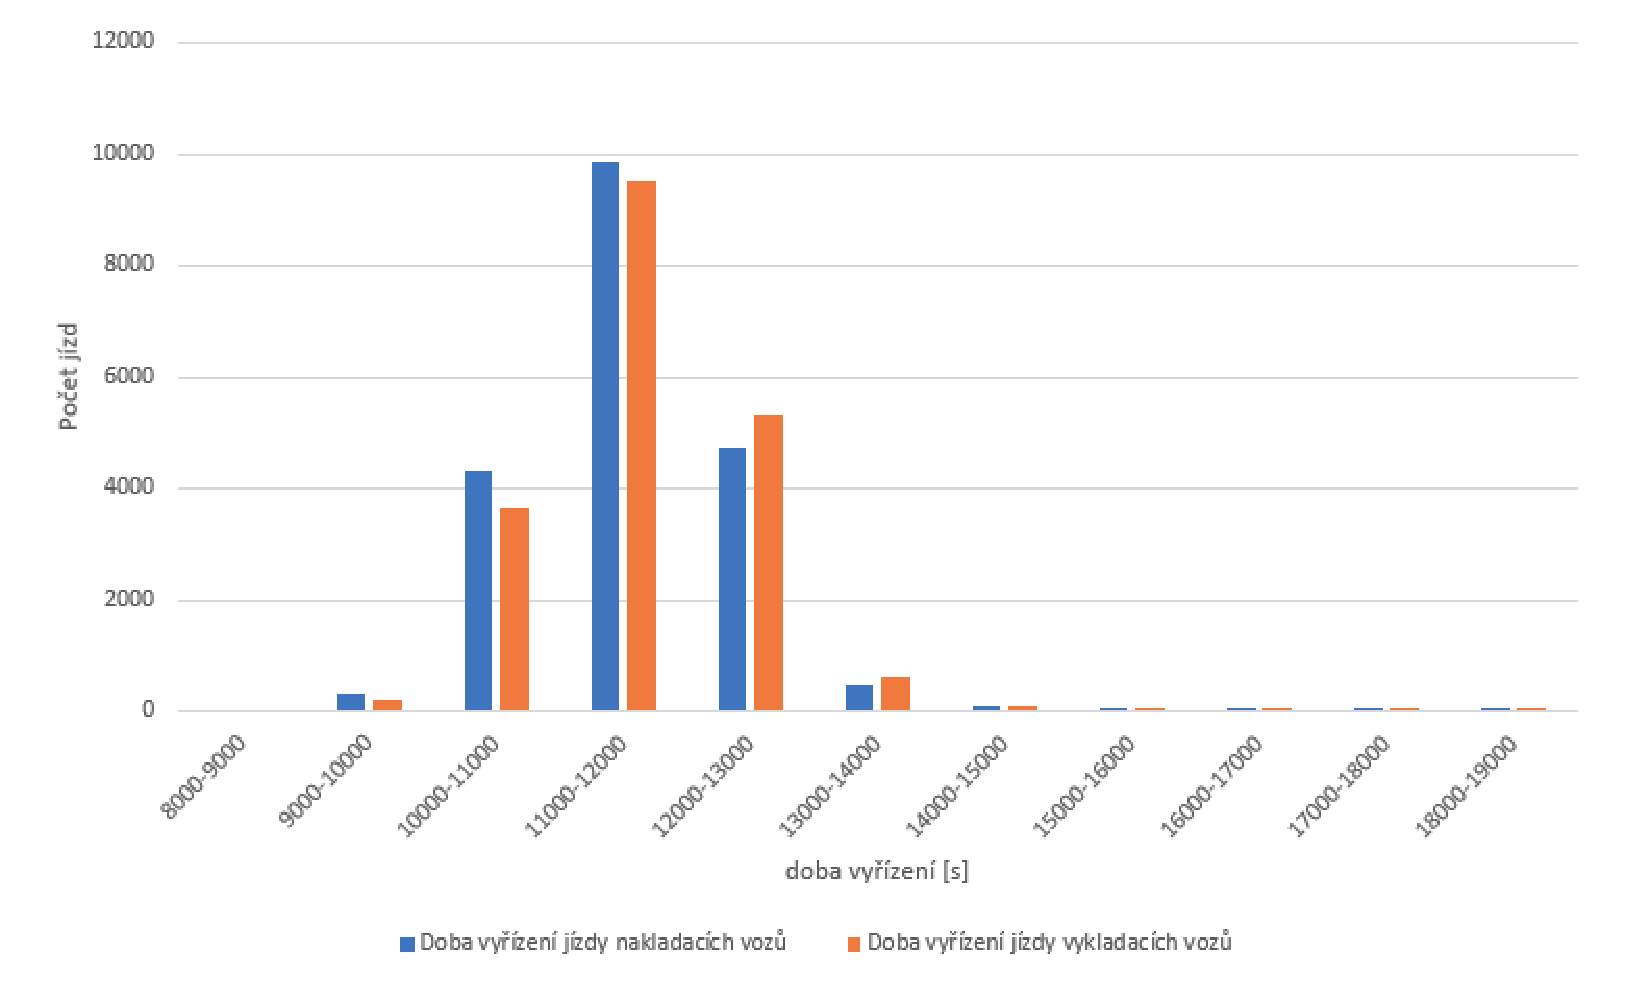
\includegraphics[scale=0.5]{exp2.eps}
\caption{Graf vyřizování jízd experimentu 2}
\end{center}
\end{figure} 

\subsubsection{Experiment 3}
\noindent V rámci experimentu číslo 3 jsme naopak zvýšili počty vozů pro všechny typy o 2. Výsledek experimentů prokázal, ze spoždení vozů v Experimentu 1 bylo způsobeno nedostatkem vozů a zvýšení jejich počtů podobné situace odstraní.\\

\begin{figure}[h!]
\begin{center}
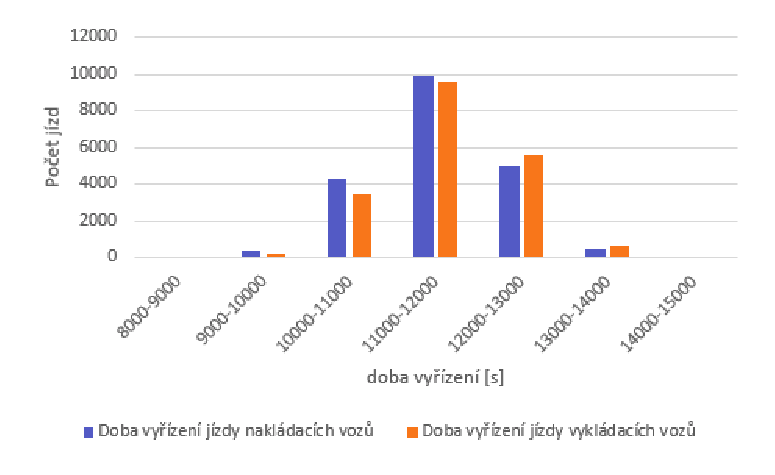
\includegraphics[scale=0.75]{exp3.eps}
\caption{Graf vyřizování jízd experimentu 3}
\end{center}
\end{figure}
\vspace{1pt}

\subsubsection{Experiment 4}
Průměrné obsazení parkoviště je nízké a tak firma uvažuje nad tím, že 4 parkovacích místa by využila jako skladište poškozených palet. V současnoti žádný z dovozních vozů nemusí odjíždět na vzdálené parkoviště. Stejnou prioritu má pro ně ale projekt nahrazení jedné vykladácí plošiny průchodem do vedlejšího skladu. Zajíma je, kolik parkovacích míst můžou po snížení počtu plošin zabrat tak, aby žádný z vozů nemusel odjet na vzdálené parkoviště. Z experimentu je patrné, 
že pokud vybudují průchod namísto plošiny, můžou pro palety vyčlenit pouze jedno parkovací místo.

\begin{figure}[h!]
\begin{center}
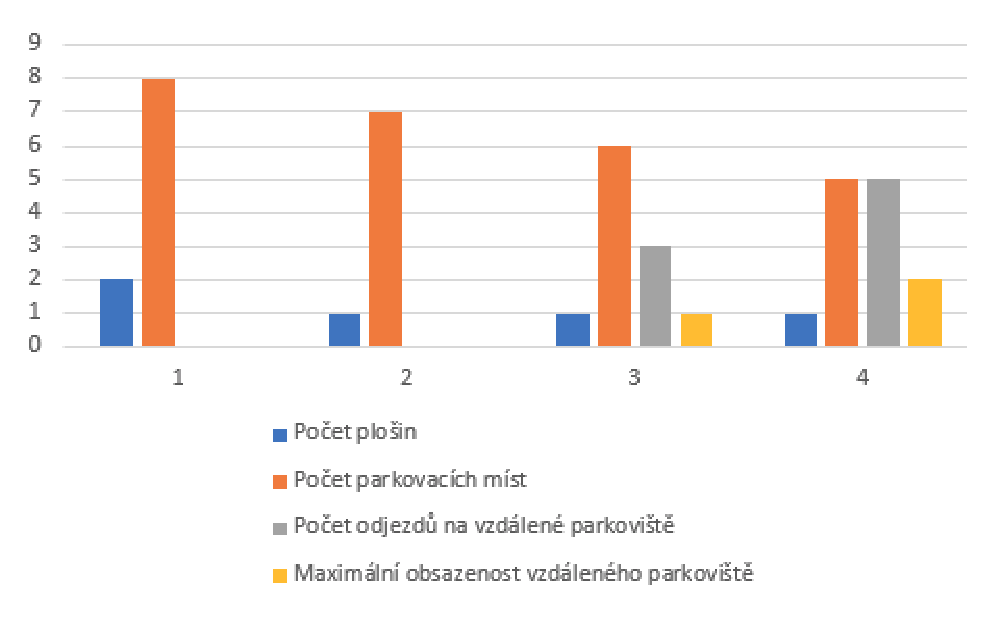
\includegraphics[scale=0.75]{exp4.eps}
\caption{Graf vyřizování jízd experimentu 4}
\end{center}
\end{figure}
\newpage

\subsubsection{Experiment 5}
Experiment 5 ukazuje chování systému po aplikaci všech změn z experimentů 3-4.
Snížil se počet vykládacích plošin, zvýšil se počet vozů a jedno místo na parkovišti se obsadilo pro skladování palet. Kombinování těchto změn vedlo k zvětšení front pro vykládací plošinu a také anulovaní benefitů získaných zvýšením počtu vozů. Pokud se ale zachová počet plošin (Obrázek 8), lze kombinovat obsazení parkoviště a zvýšení počtu vozů bez větší újmy. \\

Statistiky po aplikování všech změn:\\

Maximální fronta na vykládací plošinu: 7 \\

\begin{figure}[h!]
\begin{center}
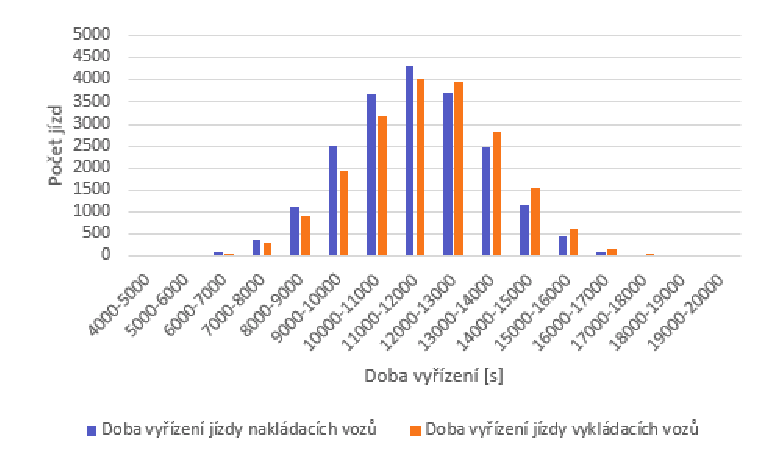
\includegraphics[scale=0.75]{exp5.eps}
\caption{Graf vyřizování jízd experimentu 5 (všechny změny)}
\end{center}
\end{figure}

Statistiky po zachování počtu plošin: \\

\begin{figure}[h!]
\begin{center}
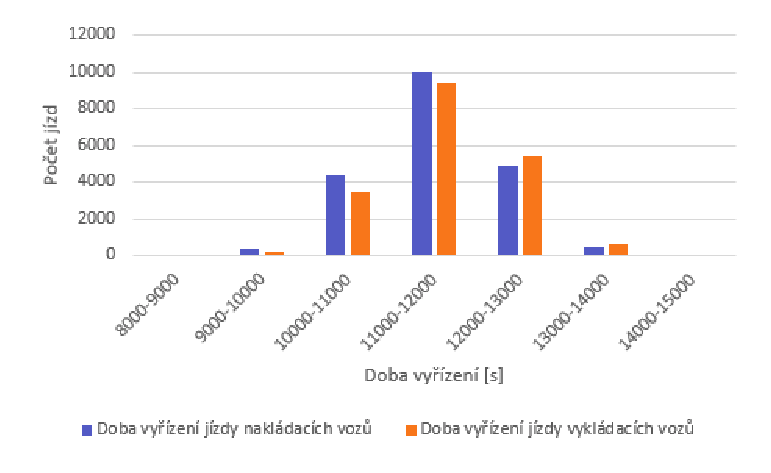
\includegraphics[scale=0.75]{exp5_2.eps}
\caption{Graf vyřizování jízd experimentu 5 (plošiny zachovány)}
\end{center}
\end{figure}
\newpage
\subsection{Závěry experimentů}
Cílem experimetování bylo zjistit, zda je možné pomocí drobných plánovaných  úprav areálu distribučního centra firmy [REDACTED] vylepšit jeho fungování. Celkem bylo provedeno 5 experimentů. Během experimentů bylo zjišteno, že pro firmu [REDACTED] za účelem odstranění dlouhých jízd se více vyplatí investovat do nových vozů než do zvýšení počtu plošin. Také se zjistilo, že pokud chce firma zachovat stav, kdy nemusí žádné vozidlo odjíždět na vzdálené parkovište a zároveň přestavět vykládací plošinu, může pro odkládání poškozených palet plánovat obsazení pouze jednoho parkovacího místa. Také se ukázalo, že firma by se měla rozhodnout, jestli zvýší počet vozů nebo sníží počet vykládacích plošin, protože kombinace těchto změn navzájem anuluje svoje výhody.

\section{Závěr}
V rámci projektu vznikl nástroj, který funguje jako simulační model distribučního centra firmy [REDACTED]. Experimentováním s tímto simulačním modelem jsme se snažili vylepšit fungování tohoto distribučního centra a poskytnout zpětnou vazbu ve formě dopadu plánovaných změn.
\newpage
\bibliographystyle{czechiso.v2}
\renewcommand{\refname}{Použité zdroje}
\bibliography{doc}
\end{document}
